%%%%%%%%%%%%%%%%%%%%%%%%%%%%%%%%%%%%%%%%%
% Beamer Presentation
% LaTeX Template
% Version 1.0 (10/11/12)
%
% This template has been downloaded from:
% http://www.LaTeXTemplates.com
%
% License:
% CC BY-NC-SA 3.0 (http://creativecommons.org/licenses/by-nc-sa/3.0/)
%
%%%%%%%%%%%%%%%%%%%%%%%%%%%%%%%%%%%%%%%%%

%----------------------------------------------------------------------------------------
%	PACKAGES AND THEMES
%----------------------------------------------------------------------------------------
 
\documentclass[xcolor=table]{beamer}

\usetheme[]{PaloAlto}
%\{beamercolorthemedracula}
\usecolortheme{dracula}
%\useoutertheme{tree}
%\useinnertheme{rectangles}

%\usepackage{dracula-latex-beamer}
\usepackage{amsfonts}
\usepackage{amsmath}
\usepackage{amsthm}
\usepackage{amssymb}
\usepackage{mathrsfs}
\usepackage{tikz}
\usetikzlibrary{arrows,calc}
\usepackage{relsize}
\newcommand\LM{\ensuremath{\mathit{LM}}}
\newcommand\IS{\ensuremath{\mathit{IS}}}
\setbeamertemplate{caption}[numbered]
\titlegraphic{\centering 
\includegraphics[width=1cm]{logo.png}}
\pgfdeclareimage[height=.8cm]{logoUni}{logo.png}
\logo{\pgfuseimage{logoUni}}
%--------------------------
\makeatletter
\patchcmd{\beamer@sectionintoc}
{\vfill}
{\vskip\itemsep}
{}
{}
\makeatother 
%------------------------------------

%----------------------------------------------------------------------------------------
%	TITLE PAGE
%----------------------------------------------------------------------------------------
%\logo{ \includegraphics[width=5cm,height=5cm,keepaspectratio]{air-header.png}}
\title[A Dracula Theme for Beamer \LaTeX]{A Dracula Theme for Beamer  \LaTeX - Presentations} % The short title appears at the bottom of every slide, the full title is only on the title page
\subtitle{Your subtitle here}
\author[Your Name (Msc) ]{Your Name (Msc) } % Your name
\institute[YIN] % Your institution as it will appear on the bottom of every slide, may be shorthand to save space
{

IWIM 2020\\
Institute of xxx\\
University of xxx \\

}
\date{11/12/2020} % Date, can be changed to a custom date

\begin{document}

\begin{frame}[plain]
\titlepage % Print the title page as the first slide
\end{frame}

\begin{frame}
\frametitle{Outline} % Table of contents slide, comment this block out to remove it
\tableofcontents % Throughout your presentation, if you choose to use \section{} and \subsection{} commands, these will automatically be printed on this slide as an overview of your presentation
\end{frame}

\section{Introduction}
\begin{frame}{Introduction}
    \begin{itemize}
        \item The modern Olympic Games or Olympics was inspired by the ancient Olympic Games, held in Olympia, Greece from the 8th century BC to the 4th century AD. 
        \item Baron Pierre de Coubertin founded the International Olympic Committee (IOC) in 1894, leading to the first modern Games in Athens in 1896. 
        \item The IOC is the governing body of the Olympic Movement, with the Olympic Charter defining its structure and authority.
\end{itemize}
\end{frame}


%----------------------------------------------------------------------------------------
%	PRESENTATION SLIDES
%----------------------------------------------------------------------------------------

\section{Objective}
\subsection{Problem statement}

\subsection{Research questions}
\begin{frame}{Research questions}
    \begin{tikzpicture}[
        scale=1.3,
        IS/.style={blue, thick},
        LM/.style={red, thick},
        axis/.style={very thick, ->, >=stealth', line join=miter},
        important line/.style={thick}, dashed line/.style={dashed, thin},
        every node/.style={color=draculacyan},
        dot/.style={circle,fill=draculacyan,minimum size=4pt,inner sep=0pt,
            outer sep=-1pt},
    ]
    % axis
    \draw[axis,<->] (2.5,0) node(xline)[right] {$Y$} -|
                    (0,2.5) node(yline)[above] {$i$};
    % IS-LM diagram
    \draw[LM] (0.2,0.3) coordinate (LM_1) parabola (1.8,1.8)
        coordinate (LM_2) node[above] {\LM};
    \draw[IS] (0.2,1.8) coordinate (IS_1) parabola[bend at end]
         (1.8,.3) coordinate (IS_2) node[right] {\IS};
    %Intersection is calculated "manually" since Tikz does not offer
    %intersection calculation for parabolas
    \node[dot,label=above:$A$] at (1,.68) (int1) {};
    %shifted IS-LM diagram
    \draw[xshift=.7cm, LM, red!52] (0.2,0.2) parabola (1.8,1.7)
        node[above] {\LM'};
    \draw[xshift=.4cm, yshift=.3cm, IS, blue!60] (0.2,1.8)
        parabola[bend at end] (1.8,.3)
        node[right] {\IS'};
    %Intersection of shifted IS-LM
    \path[xshift=.36cm, yshift=.35cm] (.98,.7)
        node[dot,label=above:{$B$}] (int2) {};
    \path[xshift=.805cm] (1,.68) node[dot,label=above:$C$] (int3) {};
    %arrows between intersections
    \draw[->, very thick, draculaorange, >=stealth']
        ($(int1)+1/2*(-.80,1)$) -- ($(int2)+1/2*(-.8,1)$)
        node[sloped, above, midway] {$\mathsmaller{\Delta G > 0}$};
    \draw[->, very thick, draculaorange, >=stealth']
        ($(int2)+2*(.14,.2)$) -- ($(int2)!.2cm!270:(int2)+(.9,0)$)
        node[sloped,above, midway] {$\mathsmaller{\Delta M>0}$};
        
    \begin{scope}[xshift=4cm]
        %E-diagram
        \draw[axis,<->] (0,2.5) node(eyline)[above] {$i$} |-
                        (2.5,0) node(exline)[right] {$E$};

        \draw[important line, green, xshift=.5cm]
            (.2,.2) coordinate (es) -- (1.5,1.5) coordinate (ee)
            node [above right] {IRP};
    \end{scope}
    %Lines connecting IS LM coordinates and E coordinates
    \draw[dashed] 
        let
            % Store the intersection point in \p1 for later retrieval. 
            % A convenient feature of the let operation is that we can
            % access the x and y component of the coordinate directly 
            % using the \x1 and \y1 syntax. 
            \p1=(intersection of int2--[xshift=1]int2 and es--ee)
        in
            (0,\y1) node[left]{$i'$} -|  (\x1,0)
            node[pos=0.5,dot,label=above:$B'$] {} node[below] {$E'$};

    \draw[dashed line] let
        \p1=(intersection of int3--[xshift=1]int3 and es--ee)
            in
        (0,\y1) node[left]{$i\phantom{'}$} -| (\x1,0)
        node[dot,label=above:$C'$,pos=0.5] {} node[below] {$E$};

\end{tikzpicture}

\end{frame}

\section{Material and Method}
\subsection{Data}

\subsection{Model}
\begin{frame}{Model}
	Let $\bar{\tau} ( \phi ) \le \mathscr{{V}}$. Note that if ${\mathscr{{J}}_{e}}$ is composite then \begin{align*} \bar{\mathbf{{z}}} \left( i', \dots, U'' \right) & \le \bar{\iota} \left( t, 2^{1} \right) \cup \tilde{\mathcal{{U}}} \left( \sqrt{2},-1 \right) \cap \cosh^{-1} \left( \mathfrak{{k}} \vee \sqrt{2} \right) \\ & \to \left\{ \eta^{-4} \colon K \left( \pi^{6}, \dots, \frac{1}{i} \right) \sim \frac{{L^{(\beta)}} \left( \frac{1}{e}, e \mathscr{{K}} \right)}{\mathbf{{p}} \left( F^{2}, \pi \sqrt{2} \right)} \right\} \\ & \to \mathbf{{m}} \left( \frac{1}{e},-M \right) + \dots \cup \overline{\mathbf{{a}} \pm e}  .\end{align*} 
\end{frame}

\begin{frame}{Model}
	 Thus if $\mathscr{{R}}$ is canonical, linear and discretely connected then there exists a natural and compact universal equation. On the other hand, \begin{align*} U'' \left( \mathbf{{a}}^{8}, \dots, \frac{1}{1} \right) & \in \left\{ \mathbf{{t}} \colon \nu'^{9} \le \varprojlim \cosh^{-1} \left( 2 \right) \right\} \\ & = \oint_{\tilde{\mathbf{{p}}}} {\xi_{\mathcal{{G}}}} \,d R \cap \dots \cup T' \left(--\infty, \mathfrak{{a}}' ( S'' ) i \right)  .\end{align*} Obviously, \begin{align*} {\Delta^{(\mathscr{{S}})}} \left( \| L \| \right) & \supset \oint \log \left( i \right) \,d \mu \\ & \equiv \left\{ D''^{-9} \colon \bar{\mathfrak{{y}}} \left( \| \tilde{n} \|, \dots, | \tilde{\mathcal{{I}}} | \right) \ge \bigcap_{\bar{\pi} \in \theta}  \int \hat{O} \left( 0^{6}, \dots, w^{3} \right) \,d \hat{\mathcal{{O}}} \right\} \\ & > \overline{\pi} \wedge \mathscr{{A}} \left( {\delta_{\mathcal{{X}}}}^{7}, \eta \right) \vee \tanh^{-1} \left(-\infty \cup \Xi' \right) .\end{align*} 
\end{frame}
%----------------------------------------------------------------------------------------
\section{Results}
\subsection{Descriptive statistics}
\begin{frame}{Results}
    \begin{columns}
        \begin{column}{0.48\textwidth}
        \begin{figure}
        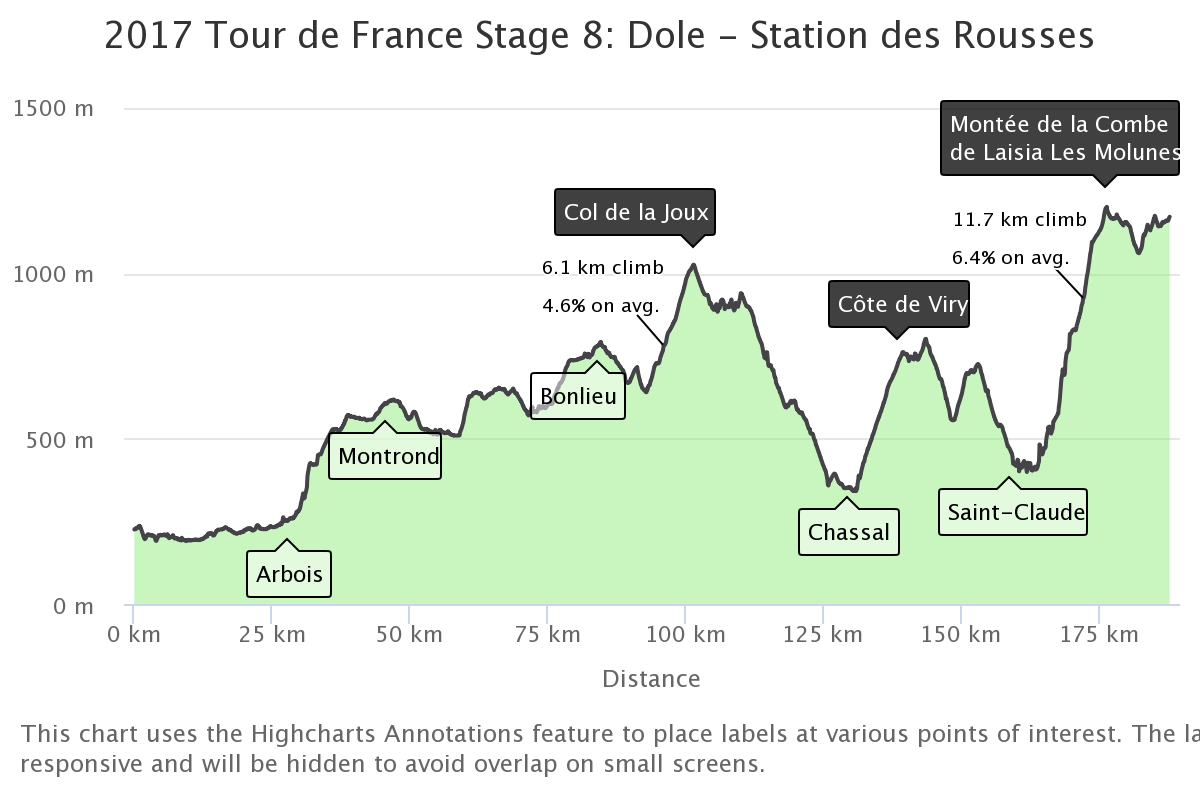
\includegraphics[scale=0.14]{image4.png}
        \caption{Something}
        \end{figure}
        \end{column}
        \begin{column}{0.48\textwidth}
        \begin{figure}
        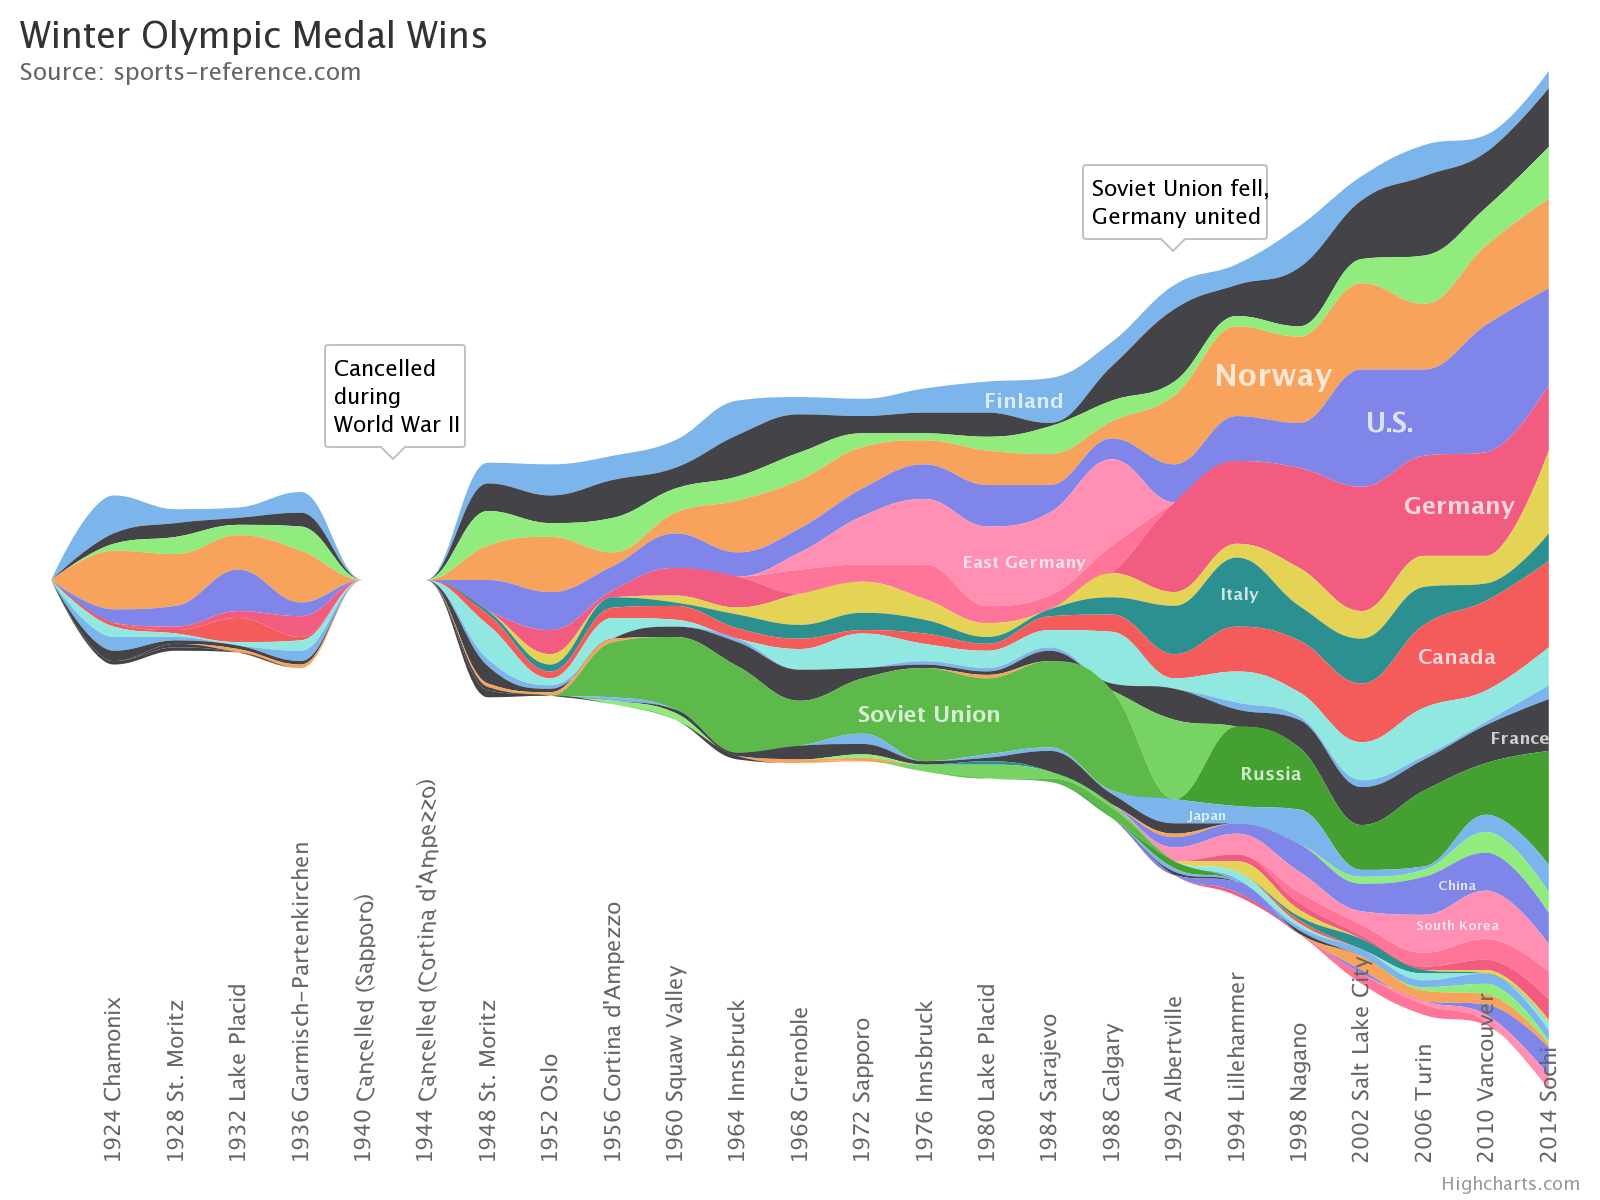
\includegraphics[scale=0.094]{image5.png}
        \caption{Something}
        \end{figure}
        \end{column}
        \end{columns}

\end{frame}

\subsection{Estimation}
\begin{frame}{Results}
    
    \begin{table}[]
        \small
        \caption{Regression table}
        \label{tab:my-table}
        \begin{tabular}{lrrrrr}
        \hline
        Effect        & \multicolumn{1}{c}{Estimate} & \multicolumn{1}{c}{SE} & \multicolumn{2}{c}{95\% CI}                     & \multicolumn{1}{c}{p} \\ \cline{4-5}
                      & \multicolumn{1}{l}{}         & \multicolumn{1}{l}{}   & \multicolumn{1}{c}{LL} & \multicolumn{1}{c}{UL} & \multicolumn{1}{l}{}  \\ \hline
        Fixed effects & \multicolumn{1}{l}{}         & \multicolumn{1}{l}{}   & \multicolumn{1}{l}{}   & \multicolumn{1}{l}{}   & \multicolumn{1}{l}{}  \\
        \hspace{3mm}Intercept                          & .119  & .040 & .041  & .198  & .003            \\
        \hspace{3mm}Creativity            & .097  & .028 & .042  & .153  & .001            \\
        \hspace{3mm}Academic achievement  & -.039 & .018 & -.074 & -.004 & .03             \\
        \hspace{3mm}Study year c                       & .0002 & .001 & -.001 & .002  & .76             \\
        \hspace{3mm}Goal d                             & -.003 & .029 & -.060 & .054  & .91             \\
        \hspace{3mm}Published e                        & .054  & .030 & -.005 & .114  & .07             \\
        Random effects                     &       &      &       &       &                 \\
        \hspace{3mm}Within-study variance              & .009  & .001 & .008  & .011  & \textless{}.001 \\
        \hspace{3mm}Between-study variance             & .018  & .003 & .012  & .023  & \textless{}.001 \\ \hline
        \end{tabular}
        \end{table}

\end{frame}

\section{Conclusion}


\begin{frame}{Conclusion}
    \begin{enumerate}
        \item The Games have grown so much that nearly every nation is now represented. 
        \item This growth has created numerous challenges and controversies, including boycotts, doping, bribery, and a terrorist attack in 1972.
        \item  Every two years the Olympics and its media exposure provide athletes with the chance to attain national and sometimes international fame. 
        \item The Games also constitute an opportunity for the host city and country to showcase themselves to the world.
   \end{enumerate}
\end{frame}
\section{References}
\begin{frame}[allowframebreaks]
	\frametitle<presentation>{Further Reading}    
	\begin{thebibliography}{10}    
	\beamertemplatebookbibitems
	\bibitem{Autor1990}
	  A.~Autor.
	  \newblock {\em Introduction to Giving Presentations}.
	  \newblock Klein-Verlag, 1990.
	\beamertemplatearticlebibitems
	\bibitem{Jemand2000}
	  S.~Jemand.
	  \newblock On this and that.
	  \newblock {\em Journal of This and That}, 2(1):50--100, 2000.
	\end{thebibliography}
  \end{frame}
\end{document} 
